
% to choose your degree
% please un-comment just one of the following
\documentclass[bsc,frontabs,twoside,singlespacing,parskip,deptreport]{infthesis}     % for BSc, BEng etc.
% \documentclass[minf,frontabs,twoside,singlespacing,parskip,deptreport]{infthesis}  % for MInf
\usepackage{listings}
\usepackage{subcaption}
\usepackage{minted}

\usepackage{graphicx}
\begin{document}

\title{High Performance Memcached}

\author{Lijing Chen}

% to choose your course
% please un-comment just one of the following
%\course{Artificial Intelligence and Computer Science}
%\course{Artificial Intelligence and Software Engineering}
%\course{Artificial Intelligence and Mathematics}
%\course{Artificial Intelligence and Psychology }   
%\course{Artificial Intelligence with Psychology }   
%\course{Linguistics and Artificial Intelligence}    
\course{Computer Science}
%\course{Software Engineering}
%\course{Computer Science and Electronics}    
%\course{Electronics and Software Engineering}    
%\course{Computer Science and Management Science}    
%\course{Computer Science and Mathematics}
%\course{Computer Science and Physics}  
%\course{Computer Science and Statistics}    

% to choose your report type
% please un-comment just one of the following
%\project{Undergraduate Dissertation} % CS&E, E&SE, AI&L
%\project{Undergraduate Thesis} % AI%Psy
\project{4th Year Project Report}

\date{\today}

\abstract{
This is an example of {\tt infthesis} style.
The file {\tt skeleton.tex} generates this document and can be 
used to get a ``skeleton'' for your thesis.
The abstract should summarise your report and fit in the space on the 
first page. 
%
You may, of course, use any other software to write your report,
as long as you follow the same style. That means: producing a title
page as given here, and including a table of contents and bibliography.
}

\maketitle

\section*{Acknowledgements}
Acknowledgements go here. 

\tableofcontents

%\pagenumbering{arabic}


\chapter{Introduction}


\section{Motivation}

Software object caches, such as Memcached, are crucial to achieving high throughput and low response latency in a datacenter setting. A well-known problem with Memcached deployments is the high overhead incurred by the kernel's TCP/IP stack in processing of individual requests. This project will evaluate the performance of a vanilla Memcached setup, followed by an assessment of the effect that user-level networking and TCP offload have on Memcached. 


\section{Project Aim}

This project is consisted of following parts.

\textbf{Baseline Tuning} We are going to first tune the original memcached and use the result as a baseline for following testing. The components we are going to tune are thread number, process number and IRQ affinity.

\textbf{User-level network Evaluation} Evaluate to what extent applying user-level networking will influence the performance of memcached.

\textbf{TCP Offload Evaluation} Evaluate the influence of multiple offloading techniques.






%
%\section{Options}
%
%There are various documentclass options, see the documentation.  Here we are
%using an option ({\tt bsc} or {\tt minf}) to choose the degree type, plus:
%\begin{itemize}
%\item {\tt frontabs} (recommended) to put the abstract on the front page;
%\item {\tt twoside} (recommended) to format for two-sided printing, with
%  each chapter starting on a right-hand page;
%\item {\tt singlespacing} (required) for single-spaced formating; and
%\item {\tt parskip} (a matter of taste) which alters the paragraph formatting so that
%paragraphs are separated by a vertical space, and there is no
%indentation at the start of each paragraph.
%\end{itemize}
%
%\chapter{Methodology}

%Of course
%you may want to use several chapters and much more text than here.









\chapter{Background}

\section{Memcached}

% reph

Memcached is a "high-performance, distributed memory object caching system, generic in nature, but intended for use in speeding up dynamic web applications by alleviating database load." Despite the official description aimed at dynamic web applications, Memcached is also used as a generic key value store to locate servers and services. 

\subsection{Memcached protocol}

Memcached support two  transport-layer protocols: TCP and UDP. They have some small difference. The basic protocol we are going to use in our experiments are described as Table~\ref{tab:mem_proto}. Note that there are many other command provided by memcached, but we are only going to test the most basic ones as listed. Comparing with TCP, the UDP protocol added an additional binary header for controlling. The binary header is described in Table~\ref{tab:mem_proto_udp}.


\begin{table}[h]
\centering
\begin{tabular}{ |p{6cm}||p{6cm}|  }

 \hline
 Operation & Description \\
 \hline
get [key]  & Get the value of given key \\
 \hline
set [key] [flags] [length] value & Set the value of given key \\
 \hline
delete [key] & delete a key provided by the argument. \\
 \hline
 
\end{tabular}
\caption{Basic Memcached protocol}
\label{tab:mem_proto}


\end{table}


\begin{table}[h]
\centering
\begin{tabular}{ |p{4cm}||p{4cm}||p{4cm}|  }

 \hline
 Position byte & Content & Description \\
 \hline
0-1  & Request ID  & The id of the request\\
 \hline
 2-3  & Sequence number  & The id of the request\\
 \hline
 4-5  & Total number of datagrams  & The id of the request\\
 \hline
 6-7  & Reserved  & Must be 0\\
 \hline

 
\end{tabular}
\caption{Memcached UDP frame header}
\label{tab:mem_proto_udp}


\end{table}




\subsection{Memcached parameters}
\label{parameter}
There are multiple parameters provided by memcached, which we can try to optimize them to get maximum performance. The parameters are listed in the Table~\ref{tab:mem_parameter} below.

\begin{table}[h]
	\centering
	\begin{tabular}{ |p{4cm}||p{8cm} |}
	
	 \hline
	 Parameter Name & Description  \\
	 \hline
	 -t or --thread  & Number of memcached thread.  \\
	 \hline
	 
	\end{tabular}
	\caption{Memcached UDP frame header}
	\label{tab:mem_parameter}
	
\end{table}


\section{User-level networking}
One performance bottleneck of modern high-performance applications is the kernel TCP/IP stack. There is a trend in industry to replace kernel TCP/IP stack with user-level TCP/IP stack.



\subsection{Data Plane Development Kit}


The Data Plane Development Kit is "a set of libraries and drivers for fast packet processing"\cite{dpdk}. It runs mostly in user-space, and it serves as a platform for developer to develop high performance networking applications.



DPDK provides developers with a framework, which contains a set of libraries for different hardware and software environments. DPDK encapsulates the low level environmental detail by creating Environment Abstraction Layer (EAL). Developers can program with a general interface, and link the library compiled for each specific environment, instead of coding with specific API from different hardware, operating systems etc.





\subsection{Seastar}
DPDK doesn't contain a TCP/IP stack. In order to migrate TCP/IP based applications to use DPDK, developers need to implement their own TCP/IP stack using DPDK provided API. 

Seastar\cite{seastar} is a framework that provided us with a ready-to-use user-level TCP/IP stack based on DPDK. Developers can use the high-level abstracted APIs provided by seastar to build high performance application without too much knowledge from low-level hardware details like EAL in DPDK.

Seastar provided a memcached for demonstration, which we are going to base our experiments on. But the demonstration memcached is not perfect, it contains multiple flaws especially when used with an open-loop tester. We will describe those issues in follow sections.



\section{TCP Offload}
TCP Offloading is another technique quite widely used in modern NIC cards. In order to alleviate the load of CPU, NIC manufacturers provided different level of offloading features in NIC, this means some of the operations like checksum, fragmentation can be processed by NIC directly instead of host CPU. 


\subsection{Full offload vs Partial offload}


There are two type of TCP Offloading. Full offload means we offload all kernel TCP/IP stack to our NIC. Partial offload means we only offload some part of TCP/IP stack to our NIC, like checksum, segmentation etc. 



% rephrase
TOE implementations also can be differentiated by the amount of processing that is offloaded to the network adapter. In situations where TCP connections are stable and packet drops infrequent, the highest amount of TCP processing is spent in data transmission and reception. Offloading just the processing related to transmission and reception is referred to as partial offloading. A partial, or data path, TOE implementation eliminates the host CPU overhead created by transmission and reception. However, the partial offloading method improves performance only in situations where TCP connections are created and held for a long time and errors and lost packets are infrequent. Partial offloading relies on the host stack to handle control—that is, connection setup—as well as exceptions. A partial TOE implementation does not handle the following:


\subsection{TCP/IP checksum offload}

% rephrase done

TCP/IP checksum offload let the network adapter to do the calculation task of verifying the checksum of packet received, which is done by CPU originally. This technique can reduce the CPU utilization.


\subsection{Large send offload}

% rephrase
Large send offload (LSO), also known as TCP segmentation offload
(TSO), frees the OS from the task of segmenting the application’s
transmit data into MTU-size chunks. Using LSO, TCP can transmit
a chunk of data larger than the MTU size to the network adapter.
The adapter driver then divides the data into MTU-size chunks and
uses the prototype TCP and IP headers of the send buffer to create
TCP/IP headers for each packet in preparation for transmission.



LSO is an extremely useful technology to scale performance
across multiple Gigabit Ethernet links, although it does so under certain
conditions. The LSO technique is most efficient when transferring
large messages. Also, because LSO is a stateless offload, it yields
performance benefits only for traffic being sent; it offers no improvements
for traffic being received. Although LSO can reduce CPU utilization
by approximately half, this benefit can be realized only if
the receiver’s TCP window size is set to 64 KB. LSO has little effect
on interrupt processing because it is a transmit-only offload.


Methods such as TCP/IP checksum offload and LSO provide limited performance gains or are advantageous only under certain conditions. For example, LSO is less effective when transmitting several smaller-sized packages. Also, in environments where packets are frequently dropped and connections lost, connection setup and maintenance consume a significant proportion of the host’s processing power. Methods like LSO would produce minimal performance improvements in such environments.



\section{Performance Analysis}

\subsection{Linux perf}

Perf is a tool provided by linux to 
Perf began as a tool for using the performance counters subsystem in Linux, and has had various enhancements to add tracing capabilities. The basic idea of perf is to set up interrupts to do sampling, the overhead is quite small if we use a reasonable sampling rate. This tool is widely used in researches about linux performance. It is a tool developed by Linux kernel team, so it can quickly adapt lastest kernel features.

\subsection{FlameGraph}
FlameGraph \cite{flamegraph} is a visualization tool for perf. We use FlameGraph for easier analysis. FlameGraph can convert perf data to bar charts and show the stack trace as stacked bars. The sample graph is attached as Figure~(todo). We can use search functionality to find out the percentage of functions we are interested in. (add sample flamegraph)







\chapter{Methodology}



\section{Quality of Service}



% rephrase

Before we start to do experiments, it's important to set up a goal for our benchmarking. For this project, a sufficient quality of service (QoS) will be under 1 millisecond for the 99th percentile request latency. 

% more BB

% Firstly, it is important the define the desired quality of service we are looking to target with our benchmarks. Frequently, distributed systems are designed to work in parallel, each component responsible for a piece of computation which is then ultimately assembled into a larger piece of response before being shipped to the client. For example, an e-commerce store may choose to compute suggested products as well as brand new products separately only to assemble individual responses into an HTML page. Therefore, the slowest of all individual components will determine the overall time required to render a response.

% Let us define the quality of service (QoS) target of this study. For our benchmarking purposes, a sufficient  QoS will be the 99th percentile tail latency of a system under 1 millisecond. This is a reasonable target as the mean latency will generally (based on latency distribution) be significantly smaller. Furthermore, it is a similar latency target used in related research.







\section{Hardware}

The Server we are using is described in  Table~\ref{tab:hardware}.


\subsection{Server}


\begin{table}[h]
\begin{tabular}{ |p{6cm}||p{6cm}|  }


 \hline
 Component Name & Device \\
 \hline
CPU & Intel(R) Xeon(R) CPU E5-2630 v4 @ 2.20GHz (40 cores) \\
 \hline
Network Interface Card & Mellanox Connect-X 4 \\
\hline
Memory & 32GB \\
 \hline
 
 
\end{tabular}
\caption{Hardware Table}
\label{tab:hardware}

\end{table}


The Network Interface Card we are using is (mlx5) \cite{P1}.


\subsubsection{Network topology}

For DPDK tests, we directly connect the NIC in two servers using network cable due to device limitation. The reason we use this topology is the NIC only supports Infiniband ports, but we don't have a switch that supports Infiniband. But then don't make a large difference and it's sufficient for us to do our experiments.






\section{Benchmark}


\subsection{Open-loop vs Closed loop}

There are two kinds of load testers: open-loop and closed-loop. Open-loop load testers send a new request only when the previous one has returned ( only one outstanding request ), while closed-loop load testers can send a new one even the previous one is pending (allow multiple outstanding requests).



\subsection{Treadmill}

Treadmill \cite{DBLP:conf/isca/ZhangMMT16} is a open-source load tester for memcached developed by Facebook. It's a typical open-loop load tester. It only supports TCP for memcached. For our experiments involving UDP, we implemented our own version of treadmill for UDP. 



\subsection{Memaslap}

Memaslap is a load tester provide by libmemcached \cite{P2}. It's a closed loop load tester.  



\chapter{Baseline Tuning}
In this chapter, we are going to tune the stock memcached by changing built-in parameters and system configurations to set up a baseline for following chapters to compare with.

\section{Multithreading}

In this section, we will evaluate how different number of threads can tail latency. Memcached supports multithreading by default, and it used spin lock % check again
for synchronization from all threads. We increase the throughput linearly find out the maximum throughput memcached can achieve when restricting the 99 percentile latency less than 1 millisecond. 


Intuitively and empirically, the best outcome we expected is when the number of memcached threads is the same as server CPU cores, as suggested by Leverich and Kozyrakis\cite{DBLP:conf/eurosys/LeverichK14},



\subsection{Setup}
The way we change the thread number is changing the argument \texttt{-t} passed to memcached. The detailed description of this parameter is mentioned in Section \ref{parameter}. 

\subsection{Result}
We can see the result in Figure~\ref{fig:threads}. According to the Figure~\ref{fig:threads}, we can see that the curve representing 4 threads (red curve) is the last one to hit the 1ms latency line, which is consistent with our previous empirical prediction. But we can also see from the figure, the 4 threads line isn't always the one with smallest latency, actually in the section from 160k throughput to 200k throughput, it's defeated by the curves representing 5 threads and 6 threads. But those two lines ("Thread 6" and "Thread 5") are getting higher latency after all 200k latency. One possible reason of this phenomenon can be CPU utilization. The curves are linearly increasing which means they are still not so close to maximum throughput, since the CPU is still under-utilized, more threads can increase some performance even they added some context switching overhead.

\begin{figure}[h]
	\centering
	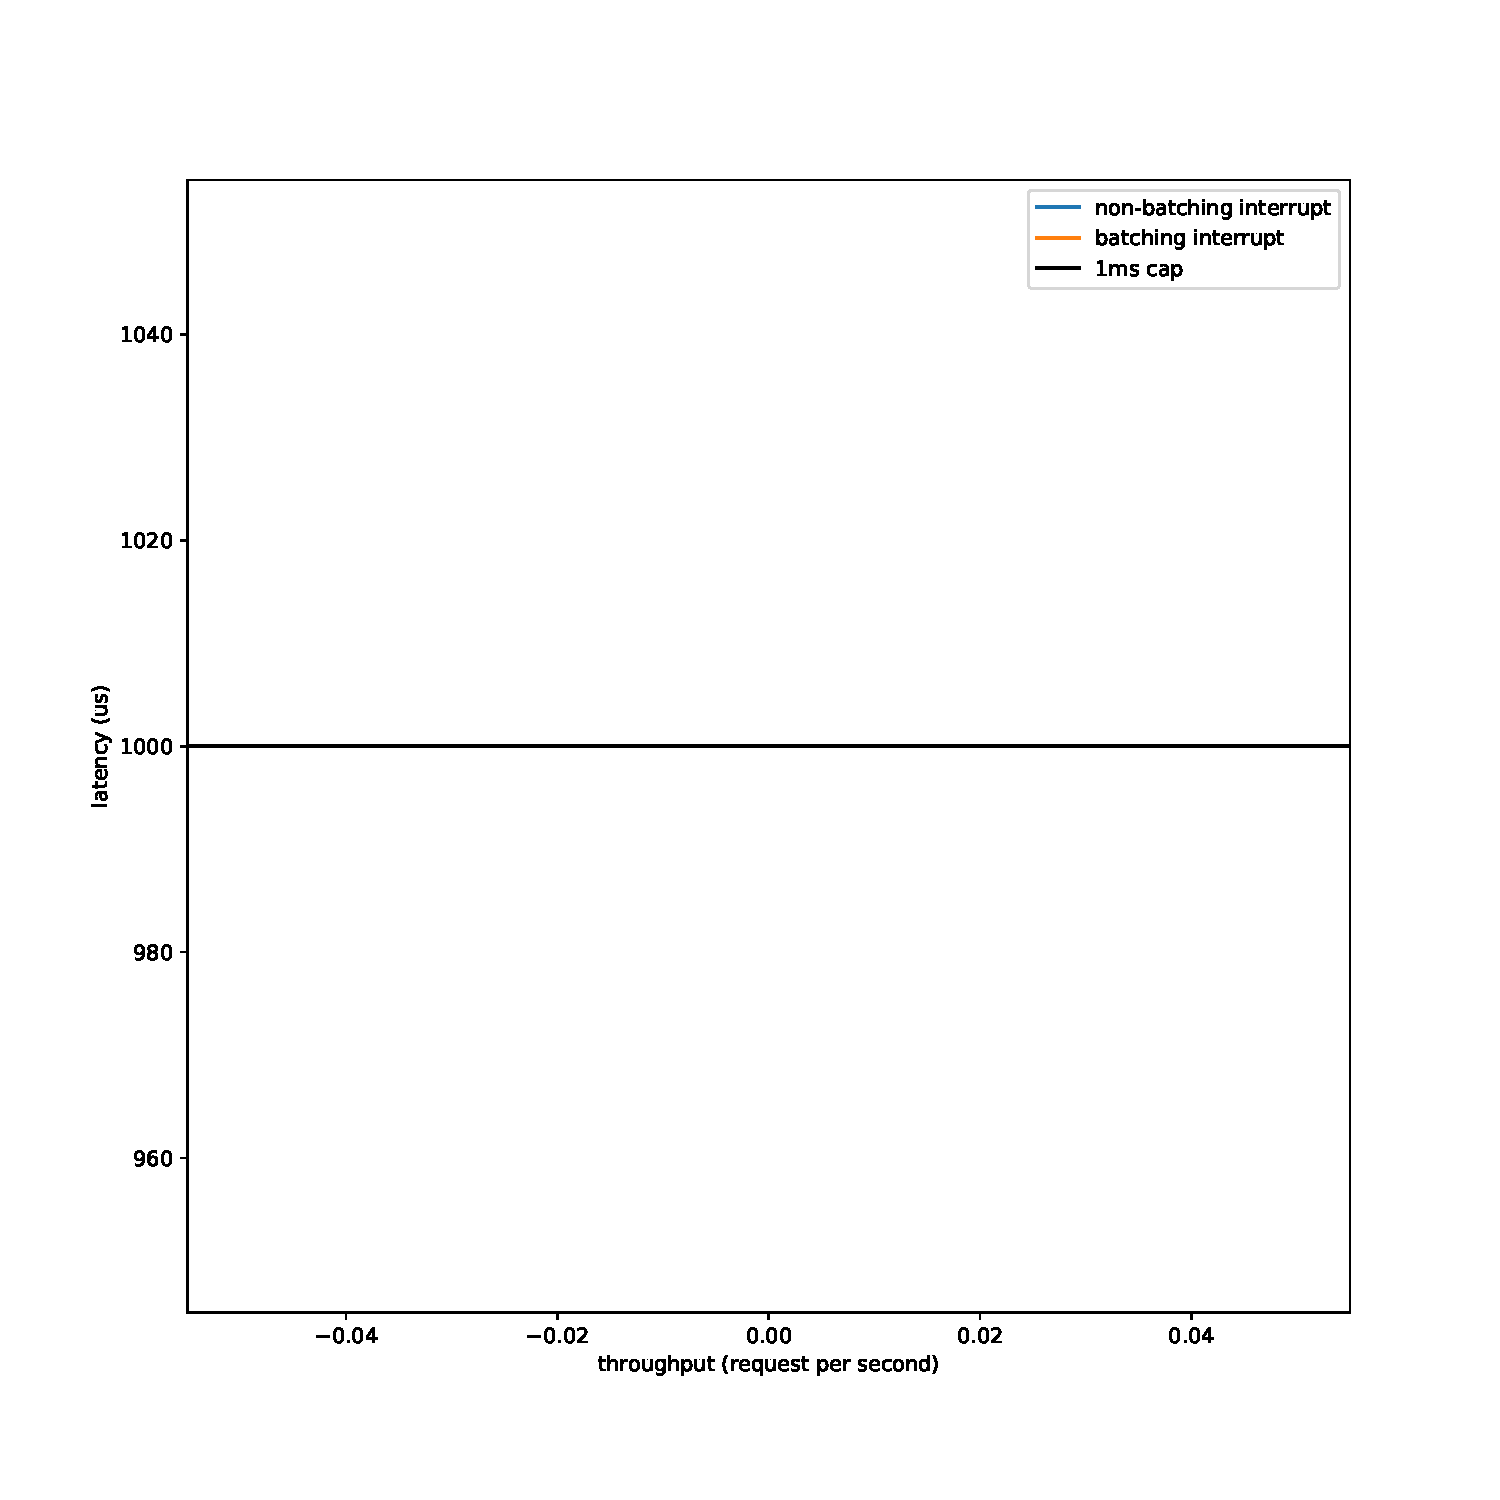
\includegraphics[width=0.7\textwidth,height=0.7\textheight,keepaspectratio]{figure/multithreading.pdf}
	\caption{Multithreading}
	\label{fig:threads}
\end{figure}






\section{Interrupt batching}
Interrupt batching is a technique for improving the performance of packet processing under heavy workload. The basic idea of interrupt batching is that instead of raising a interrupt for every packet received, batch multiple packets in one interrupt. This can significantly reduce network and CPU resources because message batching results in fewer packet to process, effectively reducing the overhead of processing a packet.

Empirically, we expect after we enabled interrupt batch, the performance have some improve.

\begin{table}
	\begin{tabular}{ |p{6cm}||p{6cm}|  }
	 \hline
	 Component Name & Device \\
	 \hline
	CPU & Intel(R) Xeon(R) CPU E5-2630 v4 @ 2.20GHz (40 cores) \\
	 \hline
	Network Interface Card & Mellanox Connect-X 4 \\
	 \hline∫
	\end{tabular}
	\caption{Hardware Table}
	\label{tab:hardware}	
\end{table}
\subsection{Setup}
We can use \texttt{ethtool} to change interrupt batching option of our NIC. The value is recommended by IBM(add cite here). The command we used is as follows.
% cite here

\begin{minted}{bash}
$ ethtool -C  p2p1 rx-usecs 5 rx-frames 5 tx-usecs 5 rx-usecs 5
\end{minted}

\begin{figure}[h]
	\centering
	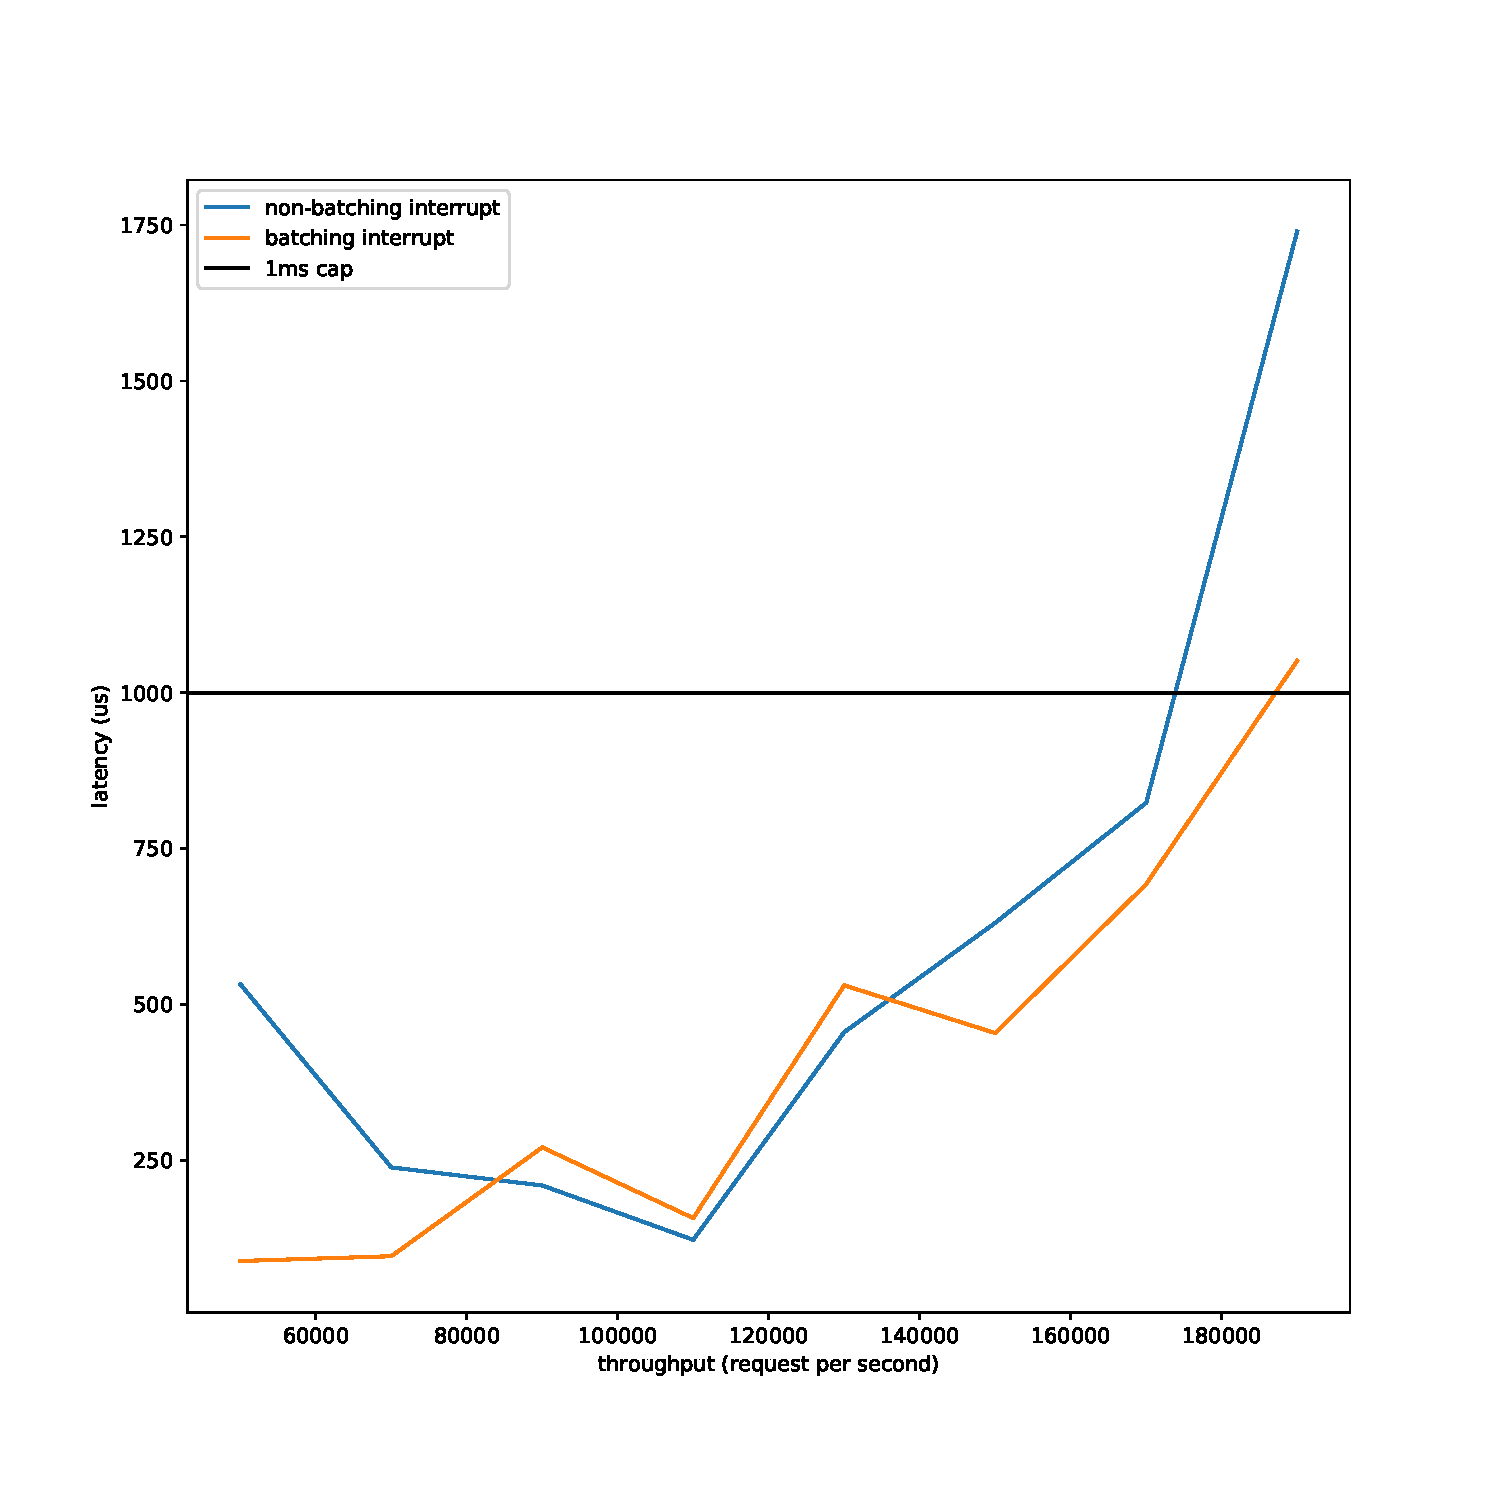
\includegraphics[width=0.7\textwidth,height=0.7\textheight,keepaspectratio]{figure/batching.pdf}
	\caption{Batching vs non-batching interrupts}
	\label{fig:batching}
\end{figure}


\subsection{Result}
% placeholder figure
The result is shown in Figure~\ref{fig:batching}. We can see that the curve representing batching interrupts can achieve a better throughput under 1ms cap than non-batching interrupts. But we can also see that in lower throughput state, not everytime batching curve can beat non-batching curve. This might because in low system utilization, batching input doesn't help that much, but the delay it brings can affect the performance. So batching interrupts does help for improving tail latency in high throughput.



\section{Multiprocessing}
In this section, we are going to use mcrouter to test the performance of multiprocessing.

\section{Setup}
We first need to setup multiple memcached instances. 

\subsection{Result}



\chapter{Contention Analysis}

\section{Core contention}

\section{SMT Thread contention}





\chapter{User-level Networking Optimization}

\section{DPDK}

\subsection{DPDK Setup}

In this section, we are going to go over how DPDK is set up.


\textbf{Setup hugepage mapping} Hugepages is a mechanism that allows the Linux kernel to utilize the multiple page size capabilities of modern hardware architectures. Linux uses pages as the basic unit of memory, where physical memory is partitioned and accessed using the basic page unit. The default page size is 4096 Bytes in the x86 architecture. Hugepages allows large amounts of memory to be utilized with a reduced overhead.



%\shellcmd{mkdir -p /mnt/huge}
%\texttt{\footnotesize\ sasasasa\newline sassasaas}

\textbf{Compile and insert DPDK kernel modules} First we need to do \texttt{make config} to tell the compiler which architecture we are targeting. We need to generate binaries working on \texttt{x86\_64-native-linuxapp-gcc}. The command is as follows.


\begin{minted}{bash}
$ make config T=x86_64-native-linuxapp-gcc
\end{minted}


Some NIC drivers are not enabled by default, including the one we are going to use (mlx5). In this case, we need to manually enable it in \texttt{ config/common\_base} file.

Then we can use \texttt{make} command to compile DPDK. After successfully compiled DPDK, switch to output folder and insert kernel module: \texttt{igb\_uio.ko}.

\begin{minted}{bash}
$ insmod igb_uio.ko
\end{minted}



\textbf{Configure NIC} First we need to unload the NIC from system kernel driver using \texttt{ifconfig}. 

\begin{minted}{bash}
$ ifconfig p2p1 down
\end{minted}

 Then we can use the tool provided by DPDK to bind NIC to kernel driver. \texttt{dpdk-devbind.py} This is common step for most NIC, but for our NIC specifically, this step is not necessary.


\section{Issues and solutions in DPDK deployment}
DOING.

\section{Experiment}
In this section, we are going evaluate the performance between DPDK implementation and stock memcached. 

\subsection{Single Core performance}
We are going to compare the latency performance DPDK memcached with stock memcached, each with only one core. The Figure~\ref{fig:dpdk_1} shows the result. 

The curve of stock memcached faded at about 200,000 rps, which means that is the maximum throughput stock memcached can achieve. We can see DPDK version can achieve a much higher maximum throughput. Also, when the throughput is the same, the DPDK one also has lower latency than stock one.

\begin{figure}[h]

	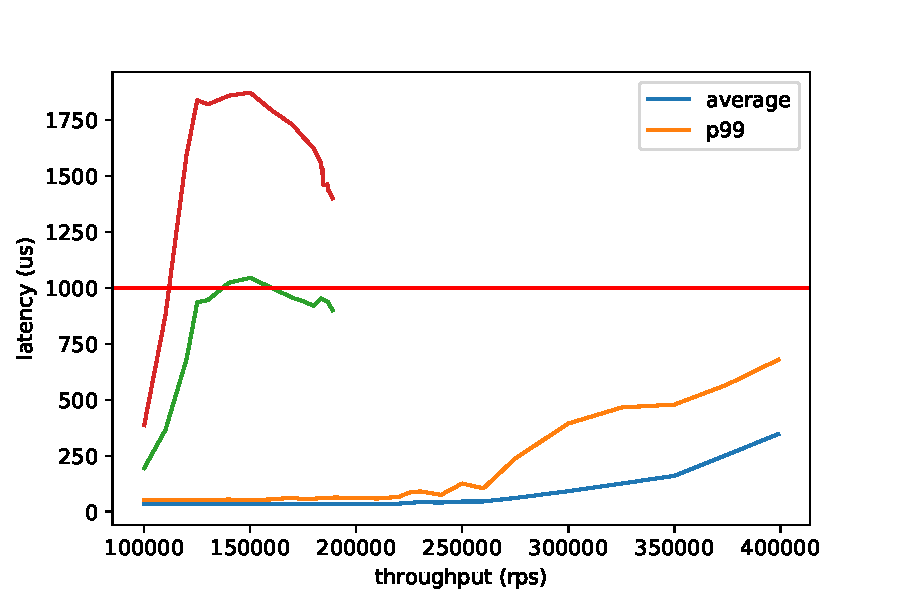
\includegraphics{figure/dpdk_1.pdf}
	\caption{DPDK}
	\label{fig:dpdk_1}
\end{figure}

\subsection{Multiple Core performance}

\section{Analysis}

\subsection{CPU utilization analysis}

One major difference between DPDK and stock is DPDK made use of its poll mode driver. Different from original interrupt based Linux kernel network stack, poll mode driver use busy waiting to avoid using interrupts, which can significantly reduce the latency. When using the poll mode driver, the CPU utilization will always be 100\%. 

We can see from Figure~\ref{fig:dpdk_busy_pie} and Figure~\ref{fig:dpdk_idle_pie_1} that in DPDK version(busy time), 99\% of time is spent in user space, while stock memcached spending 70\% time in kernel. This significantly reduce the kernel switching overhead.

\subsection{Profiling analysis}

The perf data for stock and DPDK version showed that, In the stock version, the main functionality only take up 4.89\% of run time (including pthread locking overhead), while the DPDK version spend 28.7\% in the main functionality(hashtable operation). This result reflected that the more CPU time can be used for main functionality instead of interrupt and context switching overhead. This analysis also explained the excellent performance achieved by DPDK.



%usr Show the percentage of CPU utilization that occurred while executing at the user level (application).

%sys Show the percentage of CPU utilization that occurred while executing at the system level (kernel). Note that this does not include time spent servicing hardware and software interrupts.

%iowait Show the percentage of time that the CPU or CPUs were idle during which the system had an outstanding disk I/O request.

%irq Show the percentage of time spent by the CPU or CPUs to service hardware interrupts.

%soft Show the percentage of time spent by the CPU or CPUs to service software interrupts.

%idle Show the percentage of time that the CPU or CPUs were idle and the system did not have an outstanding disk I/O request.






\begin{figure*}[t!]
    \centering
    \begin{subfigure}[t]{0.5\textwidth}
    	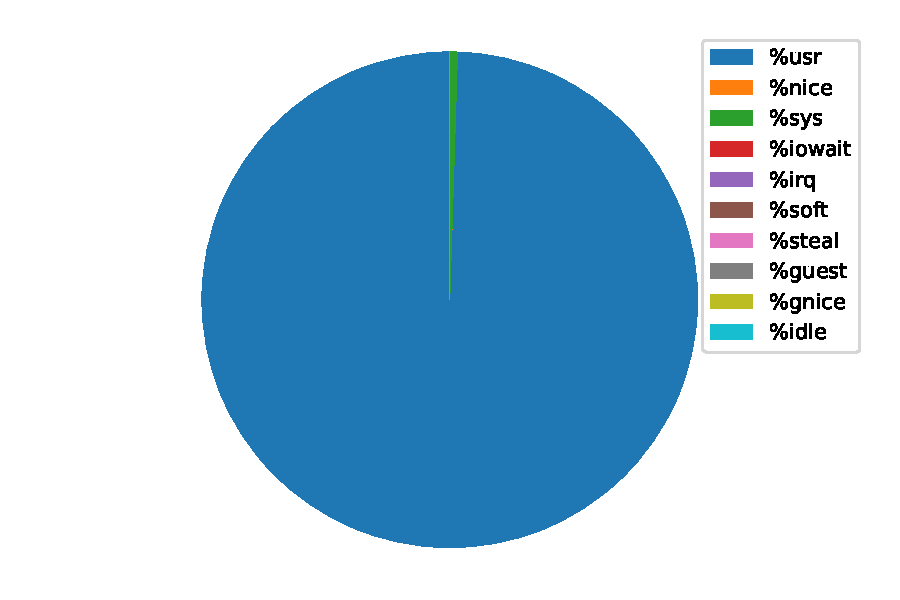
\includegraphics[height=1.5in]{figure/dpdk_busy_pie.pdf}
    	\caption{Memcached (DPDK) busy time CPU utitlization }
		\label{fig:dpdk_busy_pie}
		
    \end{subfigure}%
    ~ 
    \begin{subfigure}[t]{0.5\textwidth}
        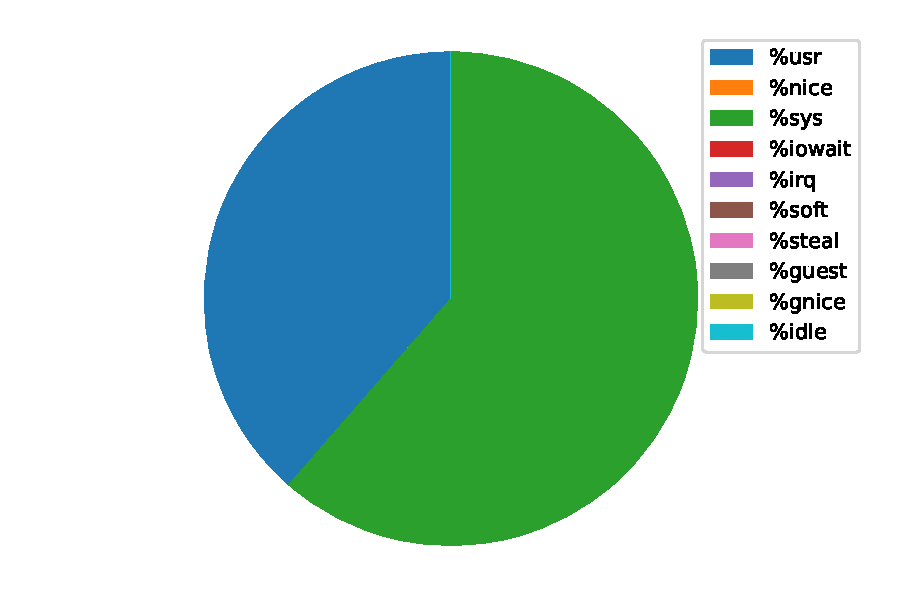
\includegraphics[height=1.5in]{figure/dpdk_idle_pie.pdf}
        \caption{Memcached (DPDK) idle time CPU utitlization}
		\label{fig:dpdk_idle_pie}
        
		
    \end{subfigure}
    \caption{DPDK CPU utilization}
\end{figure*}





\begin{figure}
	\centering
	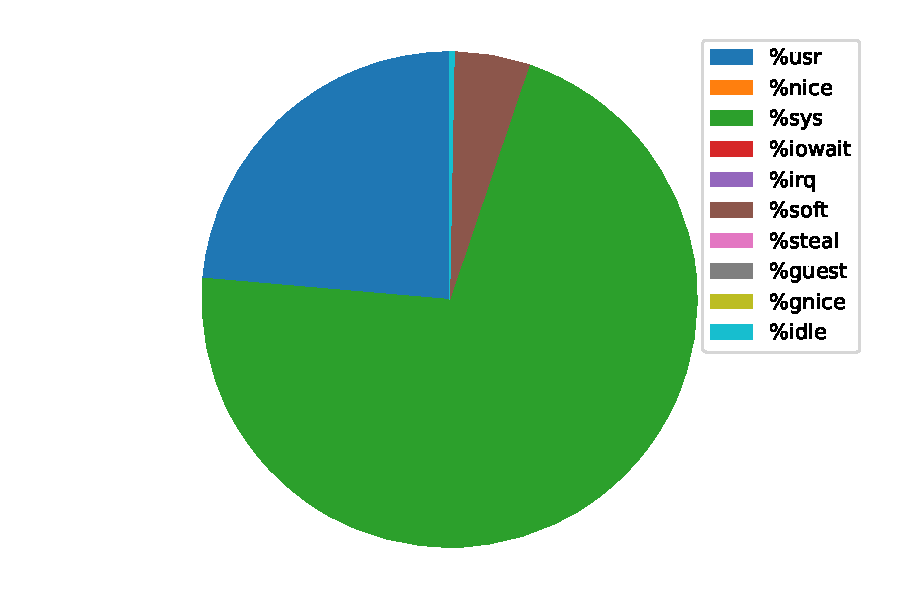
\includegraphics[width=0.5\textwidth]{figure/mem_busy_pie.pdf}
	\caption{Memcached (stock) busy time CPU utitlization}
	\label{fig:dpdk_idle_pie_1}
\end{figure}







\chapter{TCP Offloading}

\section{Setup TCP Offloading}
First, we use \textbf{ethtool} to check device offloading. We can show the support for TCP Offloading by executing following command: 
\shellcmd{ethtool -k p2p2}






%Features for p2p2:
%rx-checksumming: on
%tx-checksumming: on
%	tx-checksum-ipv4: on
%	tx-checksum-ip-generic: off [fixed]
%	tx-checksum-ipv6: on
%	tx-checksum-fcoe-crc: off [fixed]
%	tx-checksum-sctp: off [fixed]
%scatter-gather: on
%	tx-scatter-gather: on
%	tx-scatter-gather-fraglist: off [fixed]
%tcp-segmentation-offload: on
%	tx-tcp-segmentation: on
%	tx-tcp-ecn-segmentation: on
%	tx-tcp6-segmentation: on
%udp-fragmentation-offload: off [fixed]
%generic-segmentation-offload: on
%generic-receive-offload: on
%large-receive-offload: on
%rx-vlan-offload: on [fixed]
%tx-vlan-offload: on
%ntuple-filters: off [fixed]
%receive-hashing: on
%highdma: on [fixed]
%rx-vlan-filter: on
%vlan-challenged: off [fixed]
%tx-lockless: off [fixed]
%netns-local: off [fixed]
%tx-gso-robust: off [fixed]
%tx-fcoe-segmentation: off [fixed]
%tx-gre-segmentation: on
%tx-ipip-segmentation: on
%tx-sit-segmentation: on
%tx-udp_tnl-segmentation: on
%fcoe-mtu: off [fixed]
%tx-nocache-copy: off
%loopback: off
%rx-fcs: off [fixed]
%rx-all: off [fixed]
%tx-vlan-stag-hw-insert: off [fixed]
%rx-vlan-stag-hw-parse: off [fixed]
%rx-vlan-stag-filter: off [fixed]
%l2-fwd-offload: off [fixed]
%busy-poll: on [fixed]
%hw-tc-offload: off [fixed]

\section{Checksum Offload}

\subsection{Experiment}


\section{Large Send Offload}






% use the following and \cite{} as above if you use BibTeX
% otherwise generate bibtem entries
\bibliographystyle{plain}
\bibliography{mybibfile}

\end{document}
